\section*{Optical transitions in warm atomic/molecular vapors}

\begin{frame}{Working principle}

    Large scale optical transitions clocks has already shown a short-term stability $\sigma_y(\tau = 1s) \approx 10^{-18}$.
    Here, \textbf{quartz crystal local oscillator is replaced by a laser tuned to an atomic transition}.

    \vspace{10pt}

    Two different physics are exploited to reduce the Doppler broadening:

    \begin{itemize}
        \item MTS\footnotemark[1]: nonlinear interaction of laser light with atoms allows the use of a dual laser system to enable sub-Doppler spectroscopy.
        \item TPS\footnotemark[2]: shift in frequency due to moving atoms are suppressed by using two laser waves travelling in opposite directions.
    \end{itemize}

    \footnotetext[1]{MTS: Modulation transfer spectroscopy}
    \footnotetext[2]{TPS: Two-photon transitions}

\end{frame}



\begin{frame}{Two-photon transitions based clocks}

    So far, just a few optical-CSACs have been developed (experimental stage) all exploiting TPS.

    \vspace{10pt}

    NIST Chip-Scale Optical Atomic Clock (2019).

    \begin{columns}[c, onlytextwidth]

        \begin{column}{0.65\textwidth}

            \begin{figure}
                \centering
                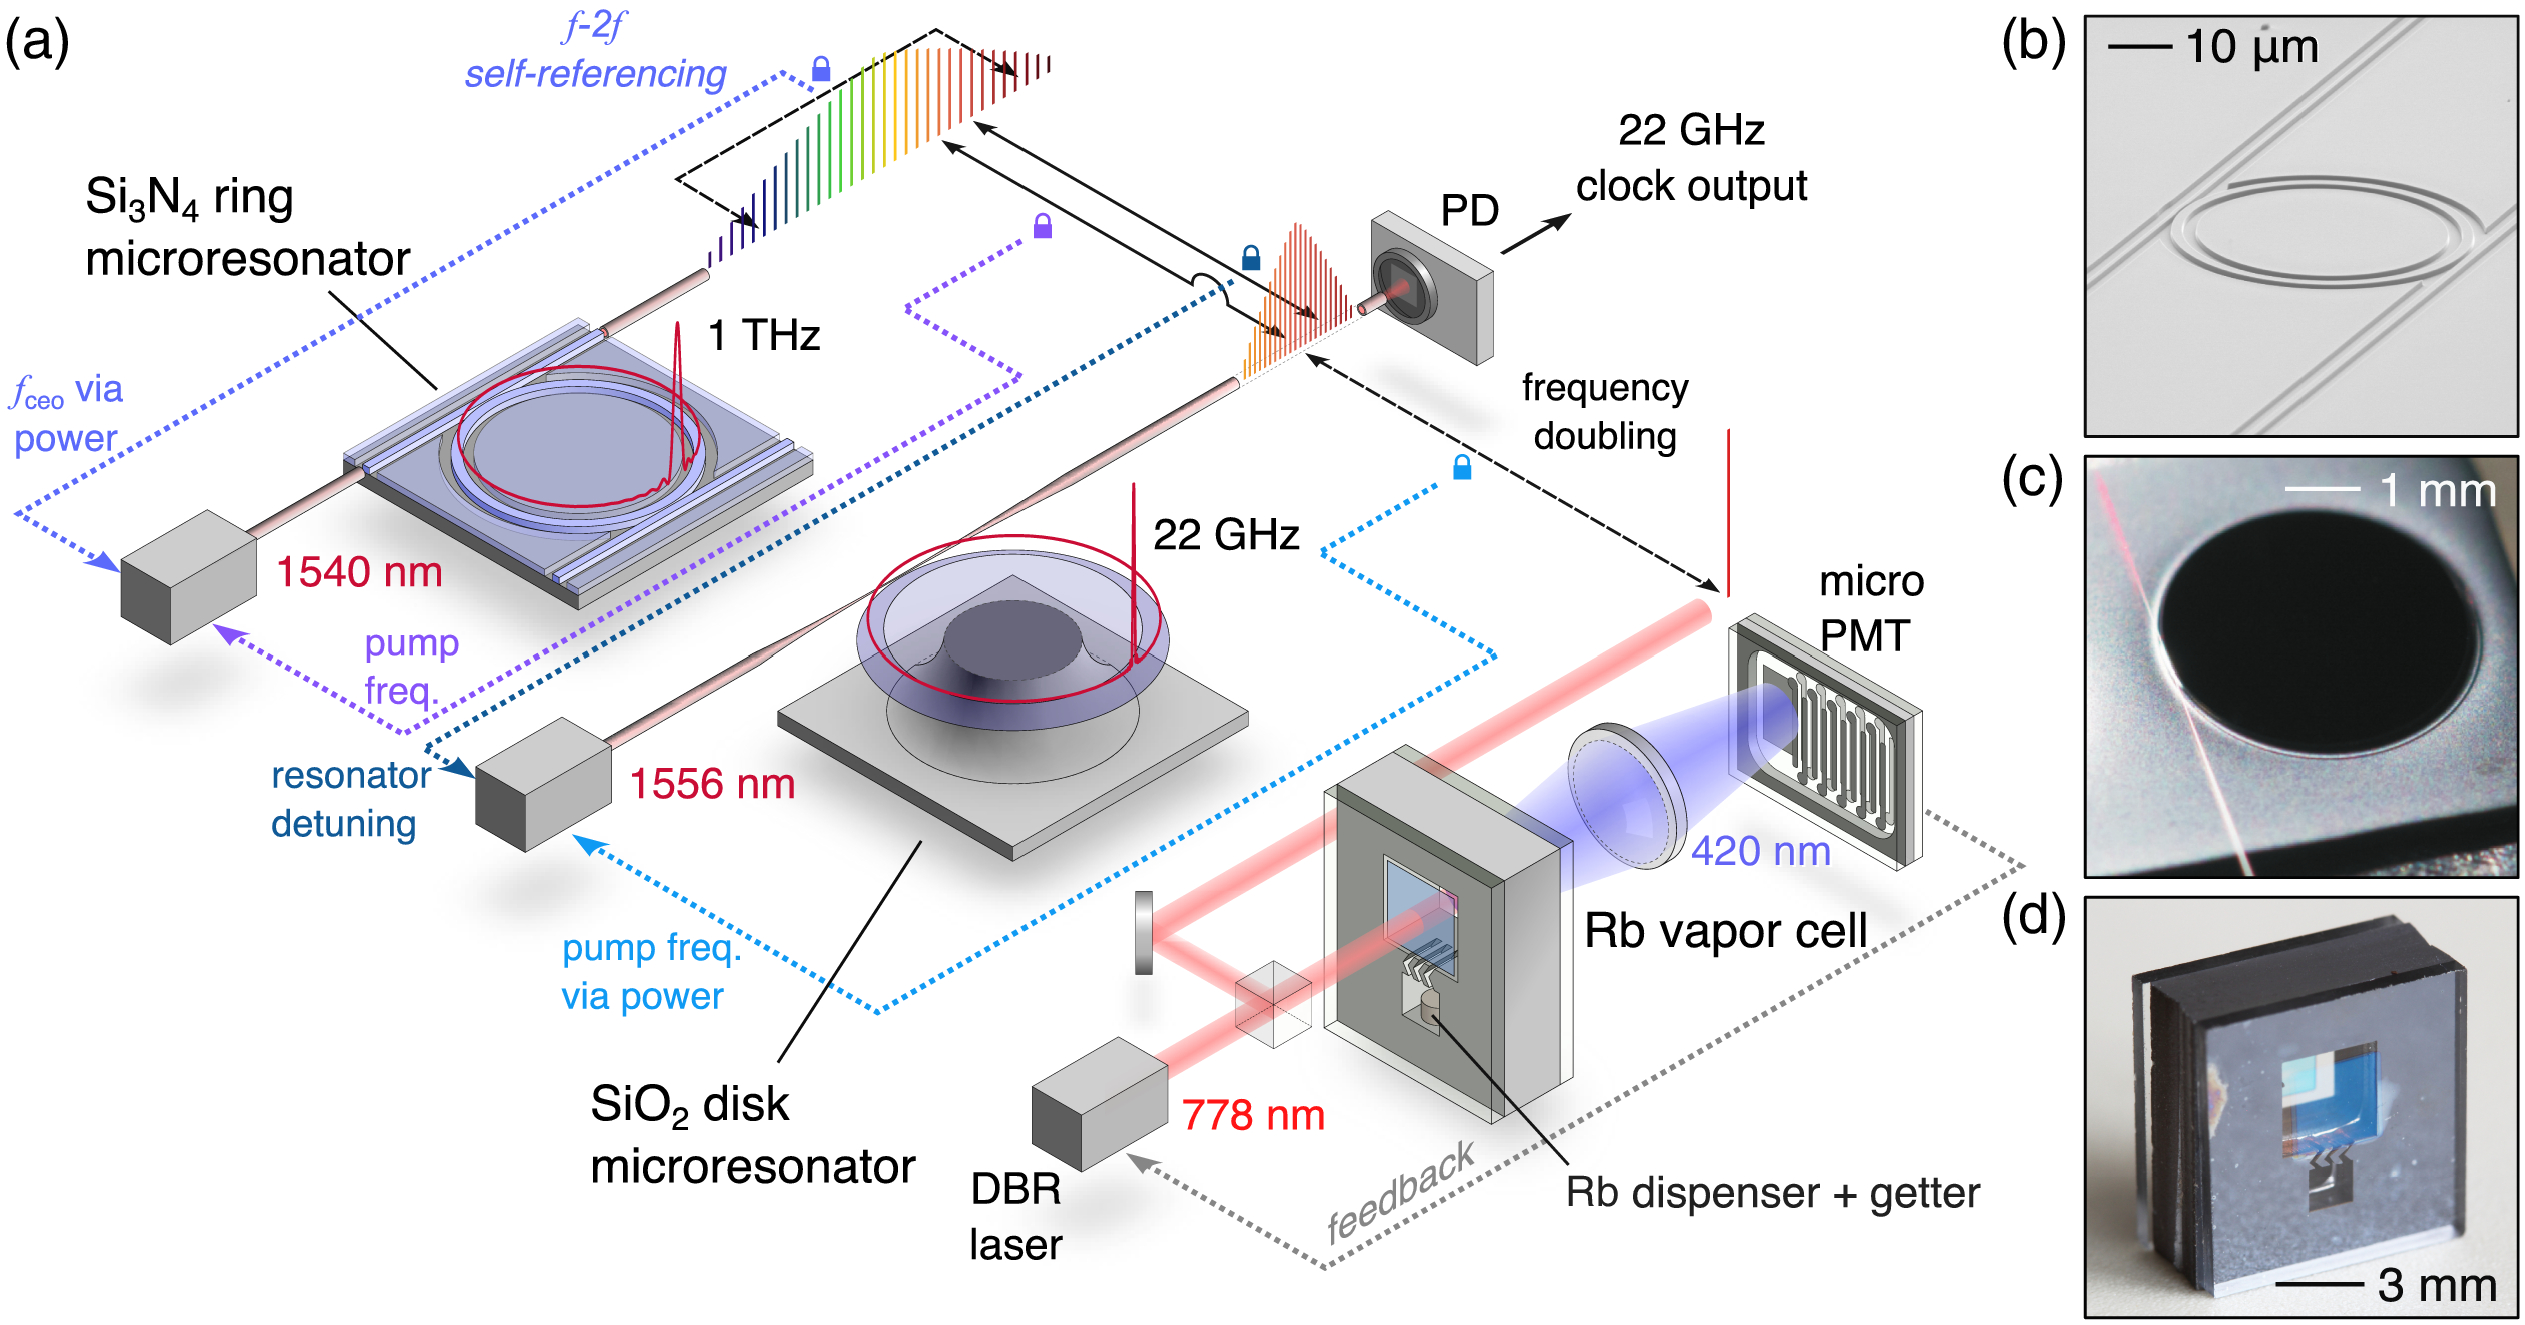
\includegraphics[width=\textwidth]{img/NIST-optical.jpeg}
            \end{figure}

        \end{column}

        \hfill

        \begin{column}{0.32\textwidth}

            Critical components:

            \begin{itemize}
                \item DBR lasers
                \item Kerr-micro-resonator frequency combs
                \item Waveguides
            \end{itemize}

        \end{column}

    \end{columns}

    \vspace{10pt}

    The \textbf{miniaturization of all the required components is the main challenge} in the optics of the NG-CSACs.

\end{frame}



\begin{frame}{Two-photon transitions based clocks}

    \begin{columns}[c, onlytextwidth]

        \begin{column}{0.5\textwidth}

            \begin{figure}
                \centering
                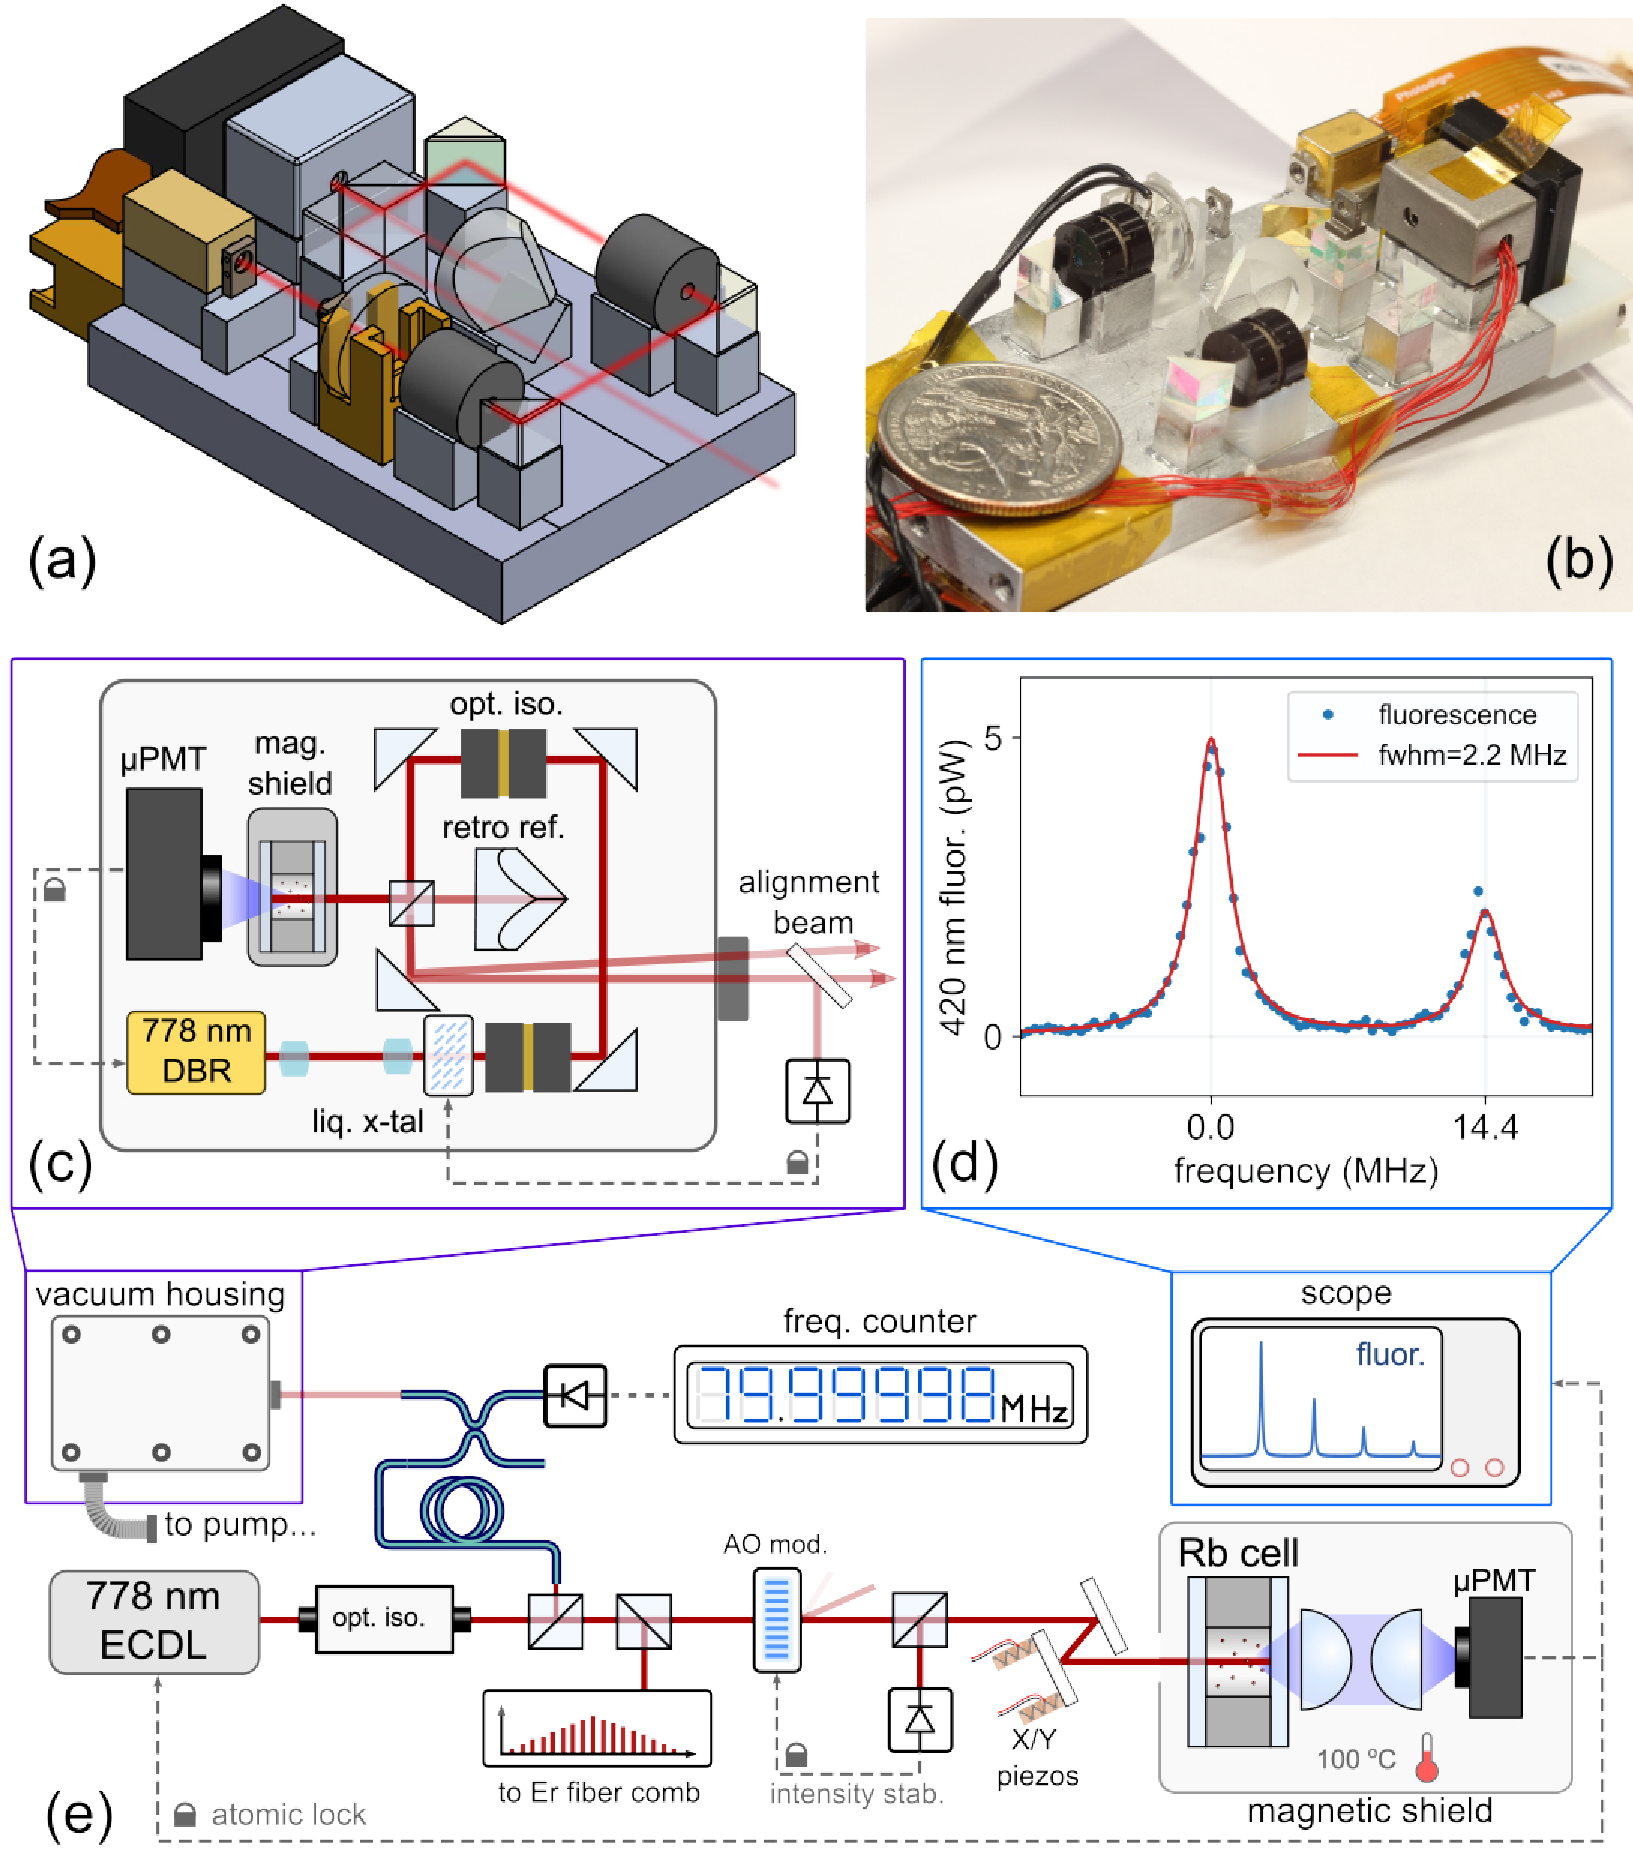
\includegraphics[width=\textwidth]{img/NIST-DRAPER-optical.jpeg}
            \end{figure}

        \end{column}

        \hfill

        \begin{column}{0.45\textwidth}

            NIST \& DRAPER optical-MAC\footnotemark[1] (2020).

            \vspace{10pt}

            Critical components:

            \begin{itemize}
                \item Microfabricated photomultiplier tubes
                \item DBR lasers
                \item Micro optics breadboards components
            \end{itemize}

        \end{column}

    \end{columns}

    \footnotetext[1]{MAC: Miniature Atomic Clock}

\end{frame}



\begin{frame}{Current results}

    Stability result shows that CSAC exploiting optical transitions met the DARPA ACES program requirements (shown in red in the figures below).

    \begin{columns}[T, onlytextwidth]

        \begin{column}{0.35\textwidth}

            \begin{figure}
                \centering
                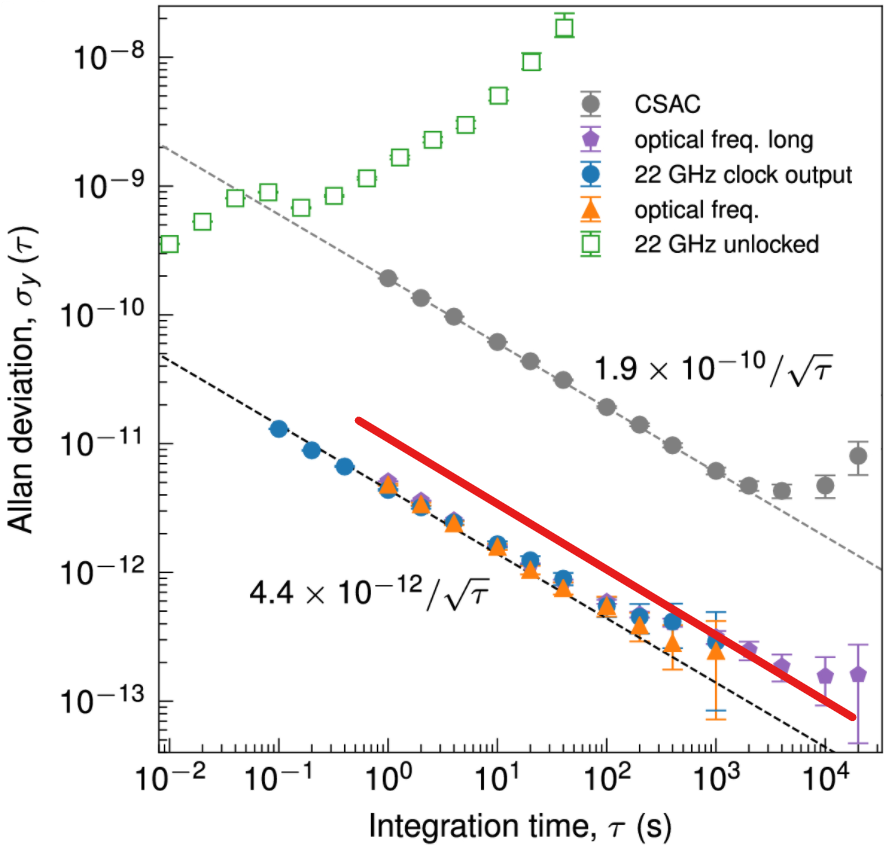
\includegraphics[width=\textwidth]{img/NIST-stability.png}
                \caption{NIST optical-CSAC stability.}
            \end{figure}

        \end{column}

        \hfill

        \begin{column}{0.55\textwidth}

            \begin{figure}
                \centering
                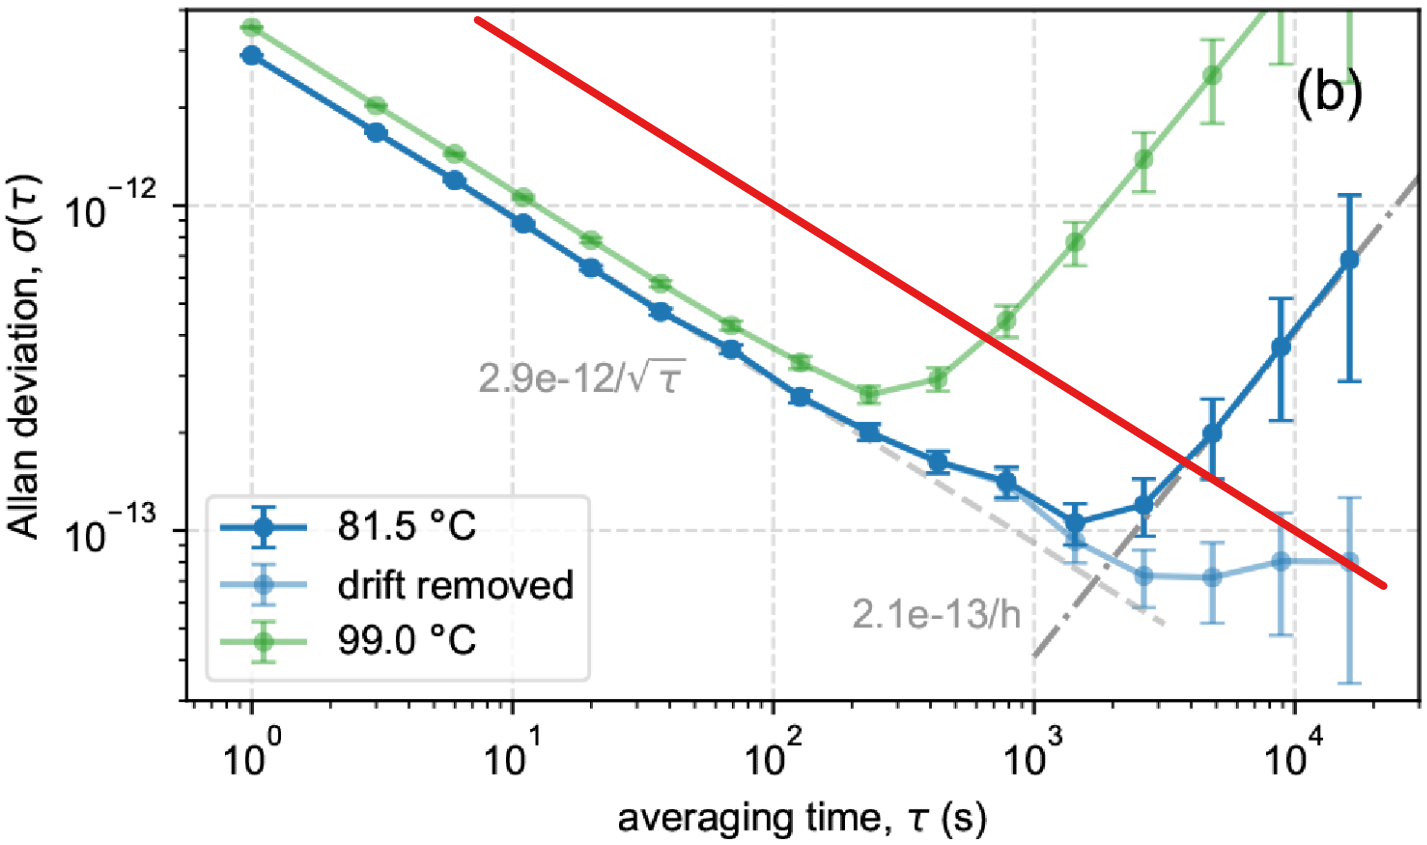
\includegraphics[width=\textwidth]{img/NIST-DRAPER-stability.png}
                \caption{NIST \& DRAPER optical-MAC stability.}
            \end{figure}
        \end{column}

    \end{columns}

    However, \textbf{the development of integrated custom micro components}, such as fast-frequency-tunable lasers and frequency microcombs, \textbf{is still a challenge}.

\end{frame}